\section{CST Model and Simulation Method}
\label{sec:model-and-method}

The model was created in CST Studio Suite Learning Edition using the planar-antenna
workflow. Geometry was defined in millimeters and frequency in GHz. The simulation
range of 0.6--1.2~GHz brackets both the 0.915~GHz design point and the final matching
minimum.

\subsection{Material and Conductor Models}

Rogers RT/duroid 5880 was represented by $\varepsilon_r=2.20$ and
$\tan\delta=0.0009$, values documented by Rogers for the laminate
\cite{rogers_5880_web,rogers_5880_datasheet}. The patch and ground conductors were
modeled as PEC. Their 0.035~mm thickness is therefore geometrical; finite copper
conductivity and conductor loss are not included.

\subsection{Final Geometry}

The patch was assembled from a main body and two inset arms, while a central feed strip
extended to the waveguide port. Figure~\ref{fig:patch-geometry} shows the preserved CST
model.

\begin{figure}[H]
    \centering
    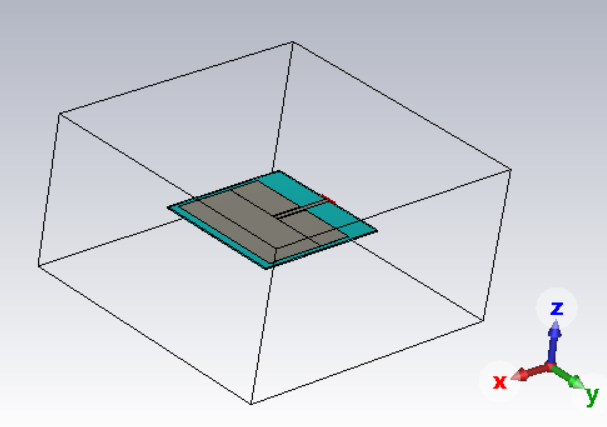
\includegraphics[width=0.64\textwidth]{figures/cst_results/fig_patch_geometry_final.png}
    \caption{Preserved CST geometry of the final inset-fed rectangular microstrip patch antenna.}
    \label{fig:patch-geometry}
\end{figure}

\begin{table}[H]
\centering
\caption{Final CST object coordinates. All dimensions are in millimeters.}
\label{tab:object-coordinates}
\resizebox{\textwidth}{!}{%
\begin{tabular}{@{}lrrrrrr@{}}
\toprule
\textbf{Object} & \textbf{$x_{\min}$} & \textbf{$x_{\max}$} & \textbf{$y_{\min}$} & \textbf{$y_{\max}$} & \textbf{$z_{\min}$} & \textbf{$z_{\max}$} \\
\midrule
Substrate & -35.0 & 118.2 & -69.75 & 69.75 & 0.000 & 1.575 \\
Ground & -35.0 & 118.2 & -69.75 & 69.75 & -0.035 & 0.000 \\
Patch body & 38.2 & 108.2 & -64.75 & 64.75 & 1.575 & 1.610 \\
Upper inset arm & 0.0 & 38.2 & 3.445 & 64.75 & 1.575 & 1.610 \\
Lower inset arm & 0.0 & 38.2 & -64.75 & -3.445 & 1.575 & 1.610 \\
Feed line & -35.0 & 38.2 & -2.445 & 2.445 & 1.575 & 1.610 \\
\bottomrule
\end{tabular}%
}
\end{table}

\subsection{Port, Boundaries, and Monitors}

A waveguide port was placed at the left substrate edge and oriented in the positive
$x$ direction. Open-add-space boundaries were used on all sides. E-field, H-field,
and far-field monitors were defined at 0.915~GHz.

\begin{table}[H]
\centering
\caption{Documented port and solver configuration.}
\label{tab:solver-configuration}
\begin{tabular}{@{}ll@{}}
\toprule
\textbf{Setting} & \textbf{Documented value} \\
\midrule
Excitation & Waveguide port 1 \\
Port plane & $x=-35$~mm \\
Port window & $y=-10$ to 10~mm; $z=-0.035$ to 4~mm \\
Propagation direction & Positive $x$ \\
Frequency range & 0.6--1.2~GHz \\
Boundary condition & Open (add space), all sides \\
Field monitors & E field, H field, far field at 0.915~GHz \\
\bottomrule
\end{tabular}
\end{table}
